\subsection{filter examples}
	\begin{frame}{filter}{typical filter types \& applications}
		\only<2>{
			\begin{figure}
				\centerline{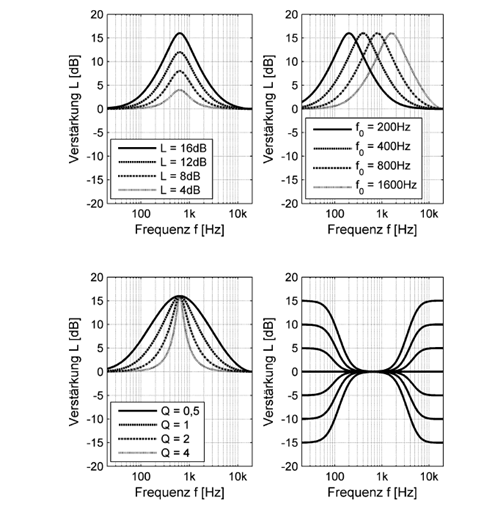
\includegraphics[scale=.5]{graph/filter}}
			\end{figure}
		}
		\only<1>{
			\begin{itemize}
				\item	\textbf{low pass \& high pass}
					\begin{itemize}
						\item	cut-off frequency, slope, (resonance)
					\end{itemize}
				\item	\textbf{low shelving \& high shelving}
					\begin{itemize}
						\item	cut-off frequency, gain
					\end{itemize}
				\item	\textbf{peak filter}
					\begin{itemize}
						\item	mid frequency, gain, bandwidth/Q
					\end{itemize}
				\item	\textbf{band pass \& bad elimination}
					\begin{itemize}
						\item	mid frequency, bandwidth/Q, slope
					\end{itemize}
				\item	\textbf{notch}
					\begin{itemize}
						\item	(mid) frequency
					\end{itemize}
			\end{itemize}
		}
        \only<3->{
        \textbf{applications} (LTI):
            \pause
            \begin{itemize}
                \item audio equalizing
                \item   removal of unnecessary/unwanted components (DC, Hum, ...)
                \item   emphasis/de-emphasis
                \item   (parameter) smoothing
            \end{itemize}
            }
	\end{frame}
	\begin{frame}\frametitle{filters}\framesubtitle{reiteration}
		\begin{table}
			\centering
%			\begin{footnotesize}
					\begin{tabular}{ccc}
					\hline
					\textbf{Z} &  & \textbf{time}\\
					\hline 
					$X(z)$ &$\leftrightarrow$& $x(i)$\\
					$X(z)\cdot z^{-k}$ &$\leftrightarrow$& $x(n-k)$\\
					\end{tabular}
%			\end{footnotesize}
		\end{table}
		\pause
		\textbf{transfer function}:
		\begin{equation*}
			H(z) = \frac{out}{in} = \frac{Y(z)}{X(z)}
		\end{equation*}
		\pause
		\textbf{spectrum}
		\begin{equation*}
			H(\jOm) = H(z\big|_{z=e^{\jOm}})
		\end{equation*}
	\end{frame}
	\begin{frame}{filters}{example 1}
	        \begin{figure}
				\begin{center}
	            \begin{picture}(50,30)
	
	                %boxes
	                \put(25,5){\framebox(7,6){\footnotesize{$z^{-1}$}}}
	
	                %lines horizontal
	                \put(5,20){\vector(1,0){22.5}}
	                \put(29.5,20){\vector(1,0){11.5}}
	                \put(43,20){\vector(1,0){10}}
	                
	                \put(15,8){\vector(1,0){10}}
	                \put(32,8){\line(1,0){10}}
	
	                %lines vertical
	                \put(15,20){\line(0,-1){12}}
	                \put(42,8){\vector(0,1){4}}
	                \put(42,14){\vector(0,1){5}}
	                
	                %circles
	                \put(27,19){$\otimes$}
	                \put(40.5,19){$\oplus$} % 42-20
	                \put(40.5,12){$\otimes$}
	                
	                \put(15,20){\circle*{1}}
	
	                %text
	                \put(26,24){\footnotesize{\shortstack[c]{$\nicefrac{1}{2}$}}}
	                \put(46,10){\footnotesize{\shortstack[c]{$\nicefrac{1}{2}$}}}
	
	                \put(4,22){\footnotesize{\shortstack[c]{x(i)}}}
	                \put(52,22){\footnotesize{\shortstack[c]{y(i)}}}
	
	            \end{picture}
				\end{center}
	        \end{figure}
        
            \only<1>{\textbf{difference equation?}}
            \pause
        	\begin{equation*}
        		y(i) = 0.5\cdot x(i) + 0.5\cdot x(i-1)
        	\end{equation*}
            \vspace{50mm}
	\end{frame}	
	
	\begin{frame}{filters}{example 1: transfer function 1/2}
    	\begin{eqnarray*}
	        		y(i) &=& 0.5\cdot x(i) + 0.5\cdot x(i-1)\\
	        		H(z) &=& 0.5  + 0.5\cdot z^{-1}\\
	       	\pause
	        		H(\jOm) &=& 0.5  + 0.5\cdot e^{-\jOm}\\
	       	\pause
	       			|H(\jOm)| &=&0.5 \cdot \left| e^{-j\frac{\Omega}{2}} \cdot \left( e^{j\frac{\Omega}{2}} + e^{-j\frac{\Omega}{2}}\right)\right| \\
	       	\pause
	       				&=&0.5 \cdot \underbrace{\left| e^{-j\frac{\Omega}{2}}\right|}_{1} \cdot  \underbrace{\left|\left( e^{j\frac{\Omega}{2}} + e^{-j\frac{\Omega}{2}}\right)\right|}_{\left| 2\cos\left(\frac{\Omega}{2}\right) \right|} \\
	       	\pause
	       	&=& \left| \cos\left(\frac{\Omega}{2}\right) \right|
    	\end{eqnarray*}
	\end{frame}	
	
	\begin{frame}{filters}{example 1: transfer function 2/2}
		\begin{figure}
			\centerline{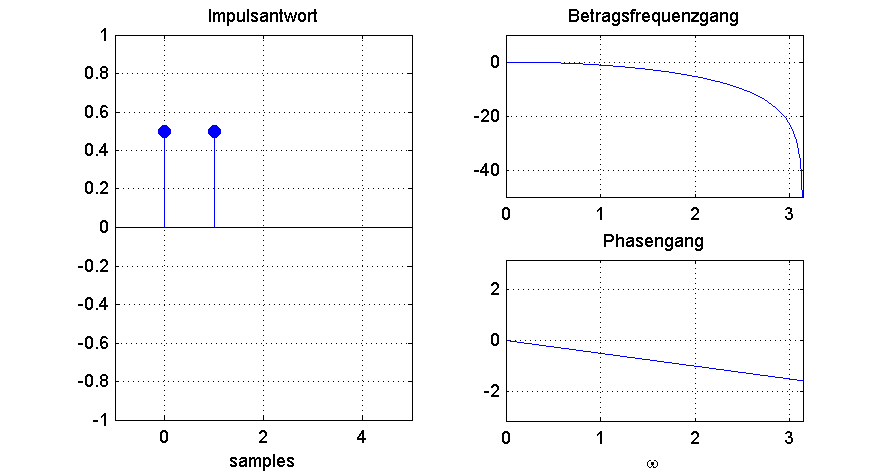
\includegraphics[scale=.7]{graph/fx_01}}
		    \label{fig:fx_01}
		\end{figure}
	\end{frame}	
	
	\begin{frame}{filters}{example 2}
        \begin{figure}
			\begin{center}
            \begin{picture}(50,30)

                %boxes
                \put(25,5){\framebox(7,6){\footnotesize{$z^{-1}$}}}

                %lines horizontal
                \put(5,20){\vector(1,0){22.5}}
                \put(29.5,20){\vector(1,0){11.5}}
                \put(43,20){\vector(1,0){10}}
                
                \put(15,8){\vector(1,0){10}}
                \put(32,8){\line(1,0){10}}

                %lines vertical
                \put(15,20){\line(0,-1){12}}
                \put(42,8){\vector(0,1){4}}
                \put(42,14){\vector(0,1){5}}
                
                %circles
                \put(27,19){$\otimes$}
                \put(40.5,19){$\oplus$} % 42-20
                \put(40.5,12){$\otimes$}
                
                \put(15,20){\circle*{1}}

                %text
                \put(26,24){\footnotesize{\shortstack[c]{$\nicefrac{1}{2}$}}}
                \put(46,10){\footnotesize{\shortstack[c]{$-\nicefrac{1}{2}$}}}

                \put(4,22){\footnotesize{\shortstack[c]{x(i)}}}
                \put(52,22){\footnotesize{\shortstack[c]{y(i)}}}

            \end{picture}
			\end{center}
        \end{figure}
            \only<1>{\textbf{difference equation?}}
            \pause
    	\begin{eqnarray*}
    		y(i) &=& 0.5\cdot x(i) - 0.5\cdot x(i-1)\\
    		H(z) &=& 0.5  - 0.5\cdot z^{-1}\\
    	\pause
    		|H(\jOm)| &=& \left| \sin\left(\frac{\Omega}{2}\right) \right|
    	\end{eqnarray*}
        \vspace{50mm}
	\end{frame}	
	
	\begin{frame}{filters}{example 2: transfer function}
		\begin{figure}
			\centerline{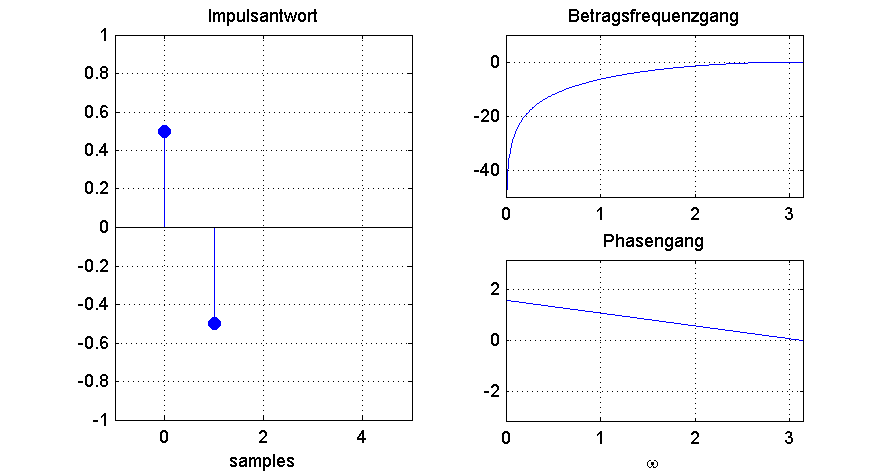
\includegraphics[scale=.7]{graph/fx_02}}
		\end{figure}
	\end{frame}	
	
	\begin{frame}{filters}{example 3}
       \begin{figure}[!hbt]
			\begin{center}
            \begin{picture}(50,30)

                %boxes
                \put(25,5){\framebox(7,6){\footnotesize{$z^{-N}$}}}

                %lines horizontal
                \put(5,20){\vector(1,0){22.5}}
                \put(29.5,20){\vector(1,0){11.5}}
                \put(43,20){\vector(1,0){10}}
                
                \put(15,8){\vector(1,0){10}}
                \put(32,8){\line(1,0){10}}

                %lines vertical
                \put(15,20){\line(0,-1){12}}
                \put(42,8){\vector(0,1){4}}
                \put(42,14){\vector(0,1){5}}
                
                %circles
                \put(27,19){$\otimes$}
                \put(40.5,19){$\oplus$} % 42-20
                \put(40.5,12){$\otimes$}
                
                \put(15,20){\circle*{1}}

                %text
                \put(26,24){\footnotesize{\shortstack[c]{$\nicefrac{1}{2}$}}}
                \put(46,10){\footnotesize{\shortstack[c]{$-\nicefrac{1}{2}$}}}

                \put(4,22){\footnotesize{\shortstack[c]{x(i)}}}
                \put(52,22){\footnotesize{\shortstack[c]{y(i)}}}

            \end{picture}
			\end{center}
        \end{figure}
            \only<1>{\textbf{difference equation?}}
            \pause
    	\begin{eqnarray*}
    		y(i) &=& 0.5\cdot x(i) - 0.5\cdot x(i-N)\\
    		H(z) &=& 0.5  - 0.5\cdot z^{-N}\\
			\pause
    		|H(\jOm)| &=& 0.5\cdot\left| e^{-j\frac{N\Omega}{2}} \cdot \left(e^{j\frac{N\Omega}{2}} - e^{-j\frac{N\Omega}{2}} \right) \right|\\
			\pause
    		 &=& \left| \sin\left(\frac{N\Omega}{2}\right) \right|
    	\end{eqnarray*}
        \vspace{50mm}
	\end{frame}	
	
	\begin{frame}{filters}{example 3: transfer function}
		\begin{figure}
			\centerline{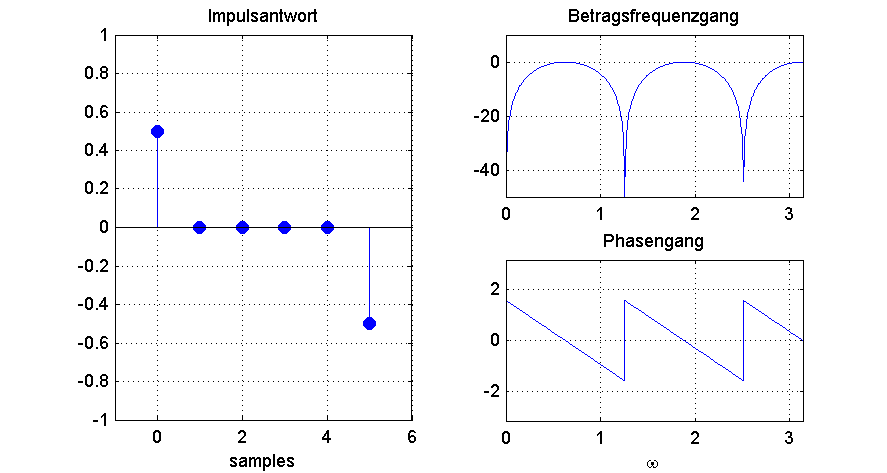
\includegraphics[scale=.7]{graph/fx_03}}
		    \label{fig:fx_03}
		\end{figure}
	\end{frame}	
	
	\begin{frame}{filters}{example 4}
        \begin{figure}
			\begin{center}
            \begin{picture}(50,70)

                %boxes
                \put(25,50){\framebox(7,6){\footnotesize{$z^{-1}$}}}
                \put(25,38){\framebox(7,6){\footnotesize{$z^{-2}$}}}
                \put(28,28){\shortstack[c]{$\vdots$}}
                \put(21,14){\framebox(14,6){\footnotesize{$z^{-(\mathcal{J}-1)}$}}}

                %lines horizontal
                \put(5,65){\vector(1,0){22.5}}
                \put(29.5,65){\vector(1,0){11.5}}
                \put(43,65){\vector(1,0){10}}
                
                \put(15,53){\vector(1,0){10}}
                \put(32,53){\vector(1,0){4}}
                \put(38,53){\vector(1,0){3}}
                
                \put(15,41){\vector(1,0){10}}
                \put(32,41){\vector(1,0){4}}
                \put(38,41){\vector(1,0){3}}
                
                \put(15,29){\vector(1,0){10}}
                \put(32,29){\vector(1,0){4}}
                \put(38,29){\vector(1,0){3}}
                
                \put(15,17){\vector(1,0){6}}
                \put(35,17){\line(1,0){7}}

                %lines vertical
                \put(15,65){\line(0,-1){48}}
                \put(42,54){\vector(0,1){10}}
                %\put(42,60){\vector(0,1){4}}
                
                \put(42,42){\vector(0,1){10}}
                %\put(42,48){\vector(0,1){4}}
                
                \put(42,30){\vector(0,1){10}}
                %\put(42,36){\vector(0,1){4}}
                
                \put(42,17){\vector(0,1){5}}
                \put(42,24){\vector(0,1){4}}
                
                %circles
                \put(27,64){$\otimes$}
                \put(40.5,64){$\oplus$} % 42-20
                \put(40.5,52){$\oplus$} % 42-20
                \put(40.5,40){$\oplus$} % 42-20
                \put(40.5,28){$\oplus$} % 42-20
                
                \put(35.5,52){$\otimes$}
                \put(35.5,40){$\otimes$}
                \put(35.5,28){$\otimes$}
                \put(40.5,22){$\otimes$}
                
                \put(15,65){\circle*{1}}
                \put(15,53){\circle*{1}}
                \put(15,41){\circle*{1}}
                \put(15,29){\circle*{1}}

                %text
                \put(26,69){\footnotesize{\shortstack[c]{$\nicefrac{1}{\mathcal{J}}$}}}
                \put(35,57){\footnotesize{\shortstack[c]{$\nicefrac{1}{\mathcal{J}}$}}}
                \put(35,45){\footnotesize{\shortstack[c]{$\nicefrac{1}{\mathcal{J}}$}}}
                \put(35,33){\footnotesize{\shortstack[c]{$\nicefrac{1}{\mathcal{J}}$}}}
                \put(44,21){\footnotesize{\shortstack[c]{$\nicefrac{1}{\mathcal{J}}$}}}

                \put(4,67){\footnotesize{\shortstack[c]{x(i)}}}
                \put(52,67){\footnotesize{\shortstack[c]{y(i)}}}

            \end{picture}
			\end{center}
        \end{figure}
        \only<1>{\textbf{difference equation?}}
        \pause
       
    	\vspace{-20mm}
    	\begin{equation*}
    		y(i) = \frac{1}{\mathcal{J}}\sum_{j=0}^{\mathcal{J}-1} x(i-j)
    	\end{equation*}
        \vspace{50mm}
	\end{frame}
	\begin{frame}{filters}{example 4: transfer function}
		\vspace{-5mm}
        \begin{figure}
			\centerline{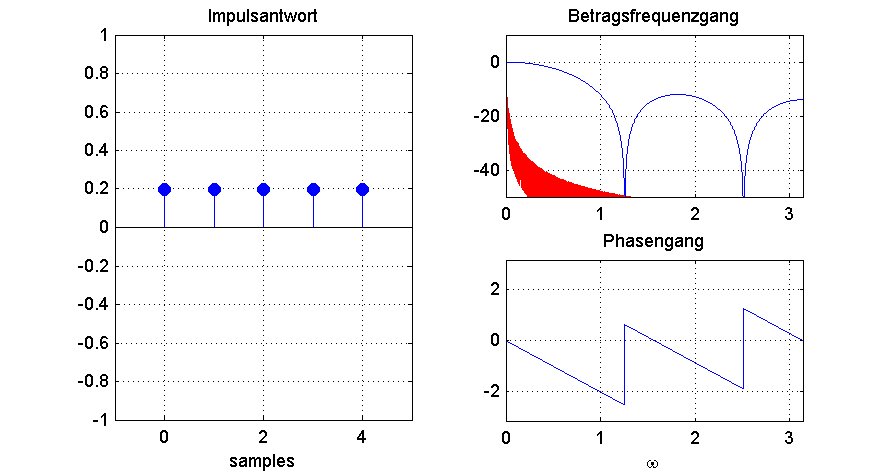
\includegraphics[scale=.7]{graph/fx_04}}
		\end{figure}
    	\begin{equation*}
    		H(\jOm) = e^{-\mathrm{j}\mathcal{J}\frac{\Omega}{2}}\frac{\sin\left(\mathcal{J}\cdot\frac{\Omega}{2} \right)}{\mathcal{J}\cdot\sin\left(\frac{\Omega}{2} \right)}
    	\end{equation*}
	\end{frame}	
	%\begin{frame}{filters}{example 4: recursive implementation}
		%\begin{eqnarray*}
			%y(i) &=& \sum\limits_{j=0}^{\mathcal{J}-1}{\frac{1}{\mathcal{J}}\cdot x(i-j)}\nonumber\\
			%\pause
			%&=& \frac{1}{\mathcal{J}}\cdot \big(x(i) - x(i-\mathcal{J})\big) + \underbrace{\sum\limits_{j=1}^{\mathcal{J}}{\frac{1}{\mathcal{J}}\cdot x(i-j)}}_{y(i-1)}\nonumber\\
			%\pause
			%&=& \frac{1}{\mathcal{J}}\cdot \big(x(i) - x(i-\mathcal{J})\big) + y(i-1) 
		%\end{eqnarray*} 
		%\pause
		%\textcolor{gtgold}{not applicable with windowed coefficients!}
	%\end{frame}
	\begin{frame}{filters}{example 5}
	        \begin{figure}[!hbt]
				\begin{center}
	            \begin{picture}(50,30)
	
	                %boxes
	                \put(25,5){\framebox(7,6){\footnotesize{$z^{-1}$}}}
	
	                %lines horizontal
	                \put(0,20){\vector(1,0){6}}
	                \put(8,20){\vector(1,0){47}}
	                
	                \put(15,8){\line(1,0){10}}
	                \put(42,8){\vector(-1,0){10}}
	
	                %lines vertical
	                \put(42,20){\line(0,-1){12}}
	                \put(15,8){\vector(0,1){4}}
	                \put(15,14){\vector(0,1){5}}
	                
	                %circles
	                \put(5.5,19){$\otimes$}
	                \put(13.5,19){$\oplus$} % 15-20
	                \put(13.5,12){$\otimes$}
	                
	                \put(42,20){\circle*{1}}
	
	                %text
	                \put(4,22){\footnotesize{\shortstack[c]{$(1-\alpha)$}}}
	                \put(11,10){\footnotesize{\shortstack[c]{$\alpha$}}}
	
	                \put(-2,22){\footnotesize{\shortstack[c]{x(i)}}}
	                \put(52,22){\footnotesize{\shortstack[c]{y(i)}}}
	
	            \end{picture}
				\end{center}
	        \end{figure}
            \only<1>{\textbf{difference equation?}}
            \pause
        	\begin{eqnarray*}
        		y(i) &=& (1-\alpha)\cdot x(i) + \alpha\cdot y(i-1)\\
        			&=& x(i) + \alpha \cdot (y(i-1) - x(i))
        	\end{eqnarray*}
            \vspace{50mm}
	\end{frame}
	
	\begin{frame}{filters}{example 5: transfer function 1/2}
    	\begin{eqnarray*}
        		y(i) &=& (1-\alpha)\cdot x(i) + \alpha\cdot y(i-1)\\
        		H(z) &=& \frac{1-\alpha}{1-\alpha z^{-1}}\\
        \pause
        		H(\jOm) &=& \frac{1-\alpha}{1-\alpha e^{-\jOm}}\\
        \pause
        		|H(\jOm)| &=& \left|\frac{1-\alpha}{1-\alpha e^{-\jOm}}\right| \\
        \pause
        		&=&\frac{1-\alpha}{\sqrt{(1 + \alpha^2 - 2\alpha\cos(\Omega)}} 
    	\end{eqnarray*}
	\end{frame}
	\begin{frame}{filters}{example 5: transfer function 2/2}
		\begin{figure}
			\centerline{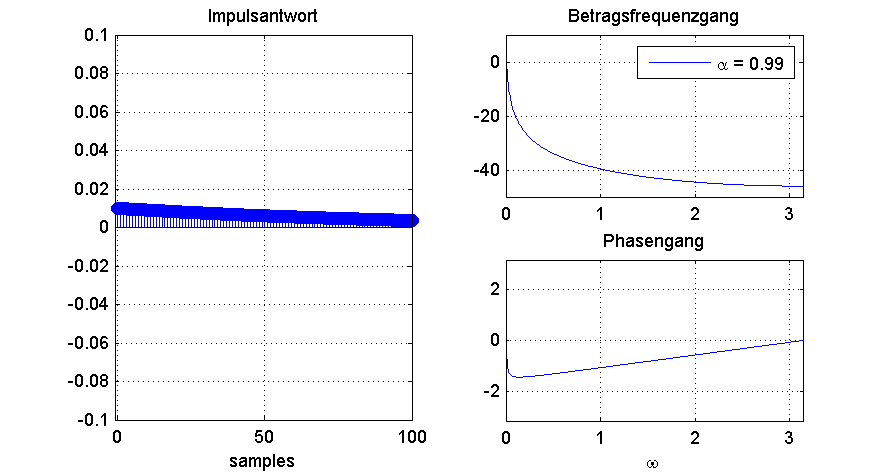
\includegraphics[scale=.7]{graph/fx_05}}
		\end{figure}
	\end{frame}
	\begin{frame}{filters}{example 6}
        \begin{figure}[!hbt]
			\begin{center}
            \begin{picture}(50,30)

                %boxes
                \put(25,5){\framebox(7,6){\footnotesize{$z^{-N}$}}}

                %lines horizontal
                \put(0,20){\vector(1,0){14}}
                \put(16,20){\vector(1,0){32}}
                \put(50,20){\vector(1,0){5}}
                
                \put(15,8){\line(1,0){10}}
                \put(42,8){\vector(-1,0){10}}

                %lines vertical
                \put(42,20){\line(0,-1){12}}
                \put(15,8){\vector(0,1){4}}
                \put(15,14){\vector(0,1){5}}
                
                %circles
                \put(47.5,19){$\otimes$}
                \put(13.5,19){$\oplus$} % 15-20
                \put(13.5,12){$\otimes$}
                
                \put(42,20){\circle*{1}}

                %text
                \put(43,22){\footnotesize{\shortstack[c]{$b_0$}}}
                \put(8,10){\footnotesize{\shortstack[c]{$-a_N$}}}

                \put(-2,22){\footnotesize{\shortstack[c]{x(i)}}}
                \put(52,22){\footnotesize{\shortstack[c]{y(i)}}}

            \end{picture}
			\end{center}
        \end{figure}
            \only<1>{\textbf{difference equation?}}
            \pause
    	\begin{equation*}
    		y(i) = b_0\cdot x(i) - a_N\cdot y(i-N)
    	\end{equation*}
        \vspace{50mm}
	\end{frame}
	\begin{frame}{filters}{example 6: transfer function}
		\vspace{-5mm}
        \begin{figure}
			\centerline{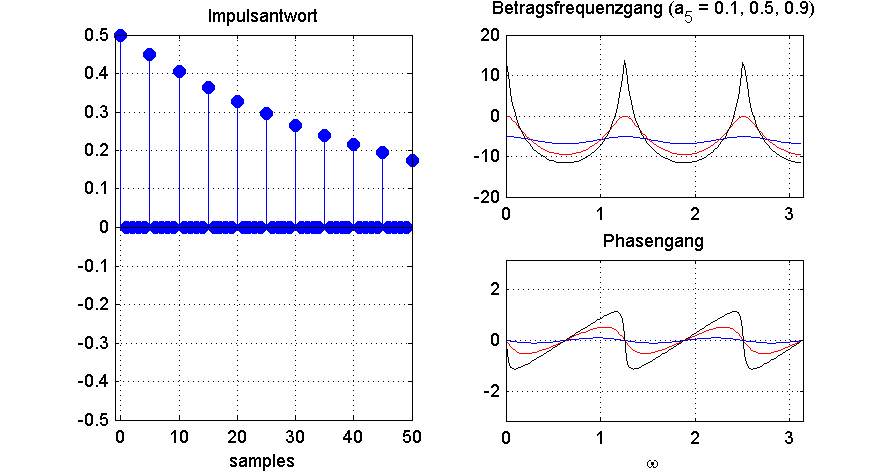
\includegraphics[scale=.7]{graph/fx_06}}
		    \label{fig:fx_06}
		\end{figure}
    	\begin{equation*}
    		H(\jOm) = \frac{b_0}{1-a_N\cdot e^{-\jOm N}}
    	\end{equation*}
	\end{frame}
	%\begin{frame}\frametitle{filters}\framesubtitle{Z-transform: example 1/2}
	        %\begin{figure}
				%\begin{center}
	            %\begin{picture}(50,30)
	%
	                %%boxes
	                %\put(25,5){\framebox(7,6){\footnotesize{$z^{-1}$}}}
	%
	                %%lines horizontal
	                %\put(0,20){\vector(1,0){6}}
	                %\put(8,20){\vector(1,0){47}}
	                %
	                %\put(15,8){\line(1,0){10}}
	                %\put(42,8){\vector(-1,0){10}}
	%
	                %%lines vertical
	                %\put(42,20){\line(0,-1){12}}
	                %\put(15,8){\vector(0,1){4}}
	                %\put(15,14){\vector(0,1){5}}
	                %
	                %%circles
	                %\put(5.5,19){$\otimes$}
	                %\put(13.5,19){$\oplus$} % 15-20
	                %\put(13.5,12){$\otimes$}
	                %
	                %\put(42,20){\circle*{1}}
	%
	                %%text
	                %\put(4,22){\footnotesize{\shortstack[c]{$(1-\alpha)$}}}
	                %\put(11,10){\footnotesize{\shortstack[c]{$\alpha$}}}
	%
	                %\put(-2,22){\footnotesize{\shortstack[c]{x(i)}}}
	                %\put(52,22){\footnotesize{\shortstack[c]{y(i)}}}
	%
	            %\end{picture}
				%\end{center}
	        %\end{figure}
	        	%\pause
	        	%\begin{eqnarray*}
	        		%y(i) &=& (1-\alpha)\cdot x(i) + \alpha\cdot y(i-1)\\
	        		%\pause
	        		%Y(z) &=& (1-\alpha)\cdot X(z) + \alpha\cdot Y(z)z^{-1}\\
	        		%\pause
	        		%H(z) &=& ?\\
	        		%\pause
	        		%|H(\jom)| &=& ?
	        	%\end{eqnarray*}
	%\end{frame}
	%\begin{frame}\frametitle{noise shaping}\framesubtitle{Z-transform: example 2/2}
	%\begin{equation*}
		%|H(\jOm)| =\frac{1-\alpha}{\sqrt{(1 + \alpha^2 - 2\alpha\cos(\Omega)}} 
	%\end{equation*}
	%\pause
	    %\begin{figure}
			%\begin{center}
				%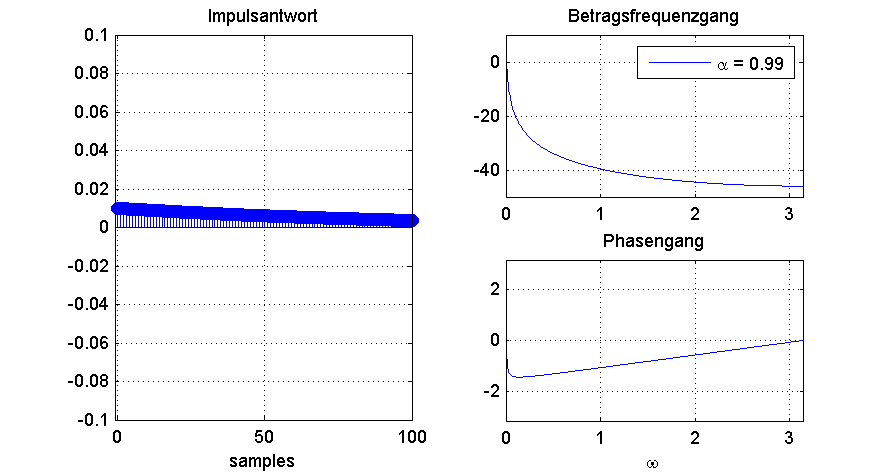
\includegraphics[scale=0.5]{Graph/fx_05}
			%\end{center}
		%\end{figure}
	%\end{frame}
\subsection{z-transform}
		\begin{frame}\frametitle{filters}\framesubtitle{biquad difference equation}
        \vspace{-5mm}
        \setlength{\unitlength}{1pt}
	        \begin{figure}[!hbt]
				\begin{center}
	            \begin{picture}(180,80)

					%%%%%%%%%%%%%%%%%%%%%%%%%%%%%%%%%%%%%%%%%%%%%%%%%%%%%%%
					%FIR	
	                %boxes
	                \put(22,47){\framebox(16,14){\footnotesize{$z^{-1}$}}}
	                \put(22,11){\framebox(16,14){\footnotesize{$z^{-1}$}}}
	
	                %lines horizontal
	                \put(19,72){\vector(1,0){37}}
	                \put(62,72){\vector(1,0){21}}
	                \put(89,72){\vector(1,0){28}}
	                
	                \put(30,38.5){\vector(1,0){26}}
	                \put(62,38.5){\vector(1,0){21.5}}
	                
	                \put(30,2.5){\vector(1,0){26}}
	                \put(62,2.5){\line(1,0){24}}
	
	                %lines vertical
	                \put(86,42){\vector(0,1){27.5}}
	                \put(30,47){\line(0,-1){9}}
	                \put(30,72){\vector(0,-1){10.5}}

	                \put(86,2.5){\vector(0,1){32.5}}
	                \put(30,11){\line(0,-1){8.5}}
	                \put(30,39){\vector(0,-1){13}}
	                
	                %circles
	                \put(55,69.5){$\otimes$}
	                \put(82,69.5){$\oplus$} 
	                \put(55,36){$\otimes$}

	                \put(82,36){$\oplus$} 
	                \put(55,0){$\otimes$}
	                
	                \put(30,72){\circle*{2}}
	                \put(30,38.5){\circle*{2}}
	
	                %text
	                \put(59,76){\footnotesize{\shortstack[c]{$b_0$}}}
	                \put(59,42.5){\footnotesize{\shortstack[c]{$b_1$}}}
	                \put(59,6.5){\footnotesize{\shortstack[c]{$b_2$}}}
	
	                \put(12,75){\footnotesize{\shortstack[c]{x(n)}}}
	                %\put(93,75){\footnotesize{\shortstack[c]{y(n)}}}


					%%%%%%%%%%%%%%%%%%%%%%%%%%%%%%%%%%%%%%%%%%%%%%%%%%%%%%%
					%IIR	
	                %boxes
	                \put(168,47){\framebox(16,14){\footnotesize{$z^{-1}$}}}
	                \put(168,11){\framebox(16,14){\footnotesize{$z^{-1}$}}}
	
	                %lines horizontal
	                %\put(89,72){\vector(1,0){37}}
	                %\put(152,72){\vector(1,0){21}}
	                \put(123,72){\vector(1,0){67}}
	                
	                \put(176,38.5){\vector(-1,0){24}}
	                \put(146,38.5){\vector(-1,0){23.5}}
	                
	                \put(176,2.5){\vector(-1,0){24}}
	                \put(146,2.5){\line(-1,0){26}}
	
	                %lines vertical
	                \put(120,42){\vector(0,1){27.5}}
	                \put(176,47){\line(0,-1){9}}
	                \put(176,72){\vector(0,-1){10.5}}

	                \put(120,2.5){\vector(0,1){32.5}}
	                \put(176,11){\line(0,-1){8.5}}
	                \put(176,39){\vector(0,-1){13}}
	                
	                %circles
	                %\put(145,69.5){$\otimes$}
	                \put(116,69.5){$\oplus$} 
	                \put(145,36){$\otimes$}

	                \put(116,36){$\oplus$} 
	                \put(145,0){$\otimes$}
	                
	                \put(176,72){\circle*{2}}
	                \put(176,38.5){\circle*{2}}
	
	                %text
	                \put(149,42.5){\footnotesize{\shortstack[c]{$-a_1$}}}
	                \put(149,6.5){\footnotesize{\shortstack[c]{$-a_2$}}}
	
	                %\put(102,75){\footnotesize{\shortstack[c]{x(n)}}}
	                \put(183,75){\footnotesize{\shortstack[c]{y(n)}}}
	
	            \end{picture}
				\end{center}
	        \end{figure}
        	\pause
            \setlength{\unitlength}{1mm}
        	\begin{eqnarray*}
        		y(i) &=& \sum\limits_{j=0}^{2}{b_j x(i-j)} - \sum\limits_{k=1}^{2}{a_j y(i-j)}\nonumber\\
        		\pause
        		Y(z) &=& \sum\limits_{j=0}^{2}{b_j X(z) z^{-j}} - \sum\limits_{k=1}^{2}{a_j Y(z) z^{-j}}\nonumber\\
        		\pause
        		Y(z)\left(1+\sum\limits_{j=1}^{2}{a_j z^{-j}}\right) &=& X(z) \sum\limits_{j=0}^{2}{b_j z^{-j}}\nonumber   		
        	\end{eqnarray*}
 		\end{frame}

		\begin{frame}\frametitle{filters}\framesubtitle{biquad: transfer function}
			\begin{eqnarray*}
				H(z) &=& \frac{Y(z)}{X(z)}\nonumber\\
				\pause
					 &=& \frac{\sum\limits_{j=0}^{2}{b_j z^{-j}}}{1+\sum\limits_{j=1}^{2}{a_j z^{-j}}}\nonumber\\
				\pause
				     &=& \frac{b_0 + b_1\cdot z^{-1} + b_2\cdot z^{-2}}{1 + a_1\cdot z^{-1} + a_2\cdot z^{-2}}\nonumber\\
					 &=&\frac{\text{numerator polynomial}}{\text{denominator polynomial}}\nonumber
					 %&=&\frac{b_0 + b_1\cdot z^{-1} + b_2\cdot z^{-2}}{(1- z_{\infty 1}\cdot z^{-1})(1- z_{\infty 2}\cdot z^{-1})}\nonumber
			\end{eqnarray*}
 		\end{frame}
		\begin{frame}\frametitle{filters}\framesubtitle{biquad: poles and zeros}
			\begin{itemize}
				\item	numerator $\rightarrow 0$: zero
				\only<1>{\item	denominator  $\rightarrow 0$: pole}
				\only<2,3,4>{\item	\textcolor{gtgold}{denominator  $\rightarrow 0$: pole}}
			\end{itemize}
			\uncover<3,4>{
				\begin{eqnarray*}
					1 + a_1\cdot z^{-1} + a_2\cdot z^{-2} &=& 0\nonumber\\
	%							z^2 + a_1\cdot z + a_2 &=& 0\nonumber
                    \pause
					\Longrightarrow z_{\infty1,2} &=& \frac{a_1}{2} \pm \frac{1}{2}\sqrt{a_1^2-4a_2}\nonumber
				\end{eqnarray*}
			}
			\uncover<4>{
				stability:
					\begin{equation}\nonumber
						|z_{\infty1,2}| < 1
					\end{equation}
				
			}
			%Beispielrechnung Instabilit�t
		\end{frame}
		\begin{frame}\frametitle{filters}\framesubtitle{biquad: zplane example}
				\begin{figure}[!hbt]
					\begin{center}
						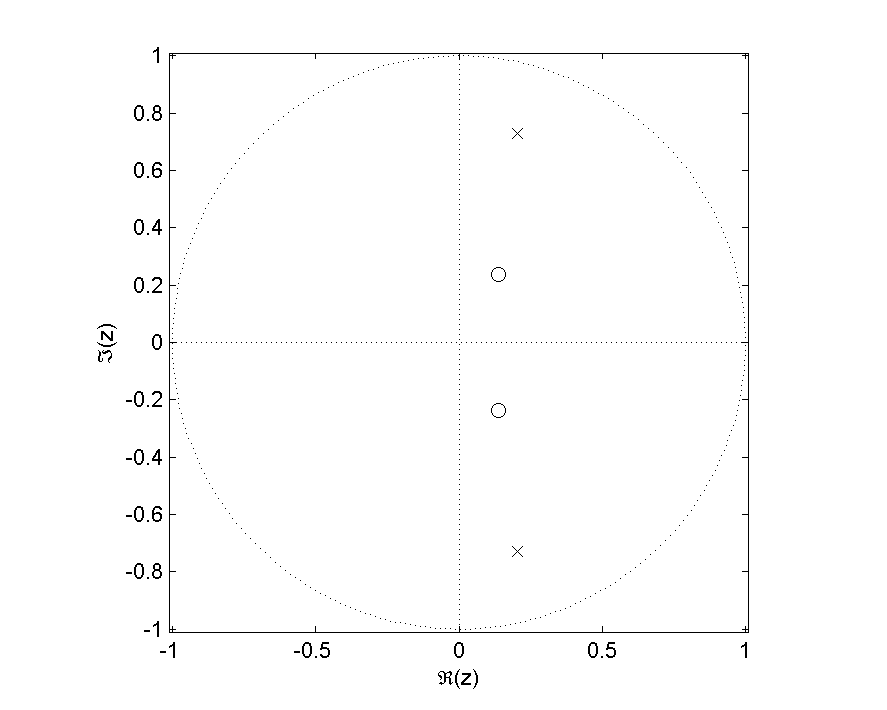
\includegraphics[scale=.6]{graph/PoleZero}
					\end{center}
				\end{figure}
		\end{frame}
		\begin{frame}\frametitle{filters}\framesubtitle{biquad: animation}
            %\vspace{-5mm}
            %\hspace*{-20mm}
            %\animategraphics[scale=.4,autoplay,loop]{10}{graph/BiquadPoleZero/BqPZ_}{1}{100}       
            \hspace*{-25mm}\includemedia[
                        addresource=video/BqPZ.mp4,
                        width=1.436\linewidth,
                        height=0.6\linewidth,
                        activate=onclick,
                        flashvars={
                            source=video/BqPZ.mp4  
                            &autoPlay=true
                        }]
                        {}
                        {VPlayer.swf}
 		\end{frame}
		\begin{frame}\frametitle{filters}\framesubtitle{biquad: z-transform}
				\begin{figure}[!hbt]
					\begin{center}
						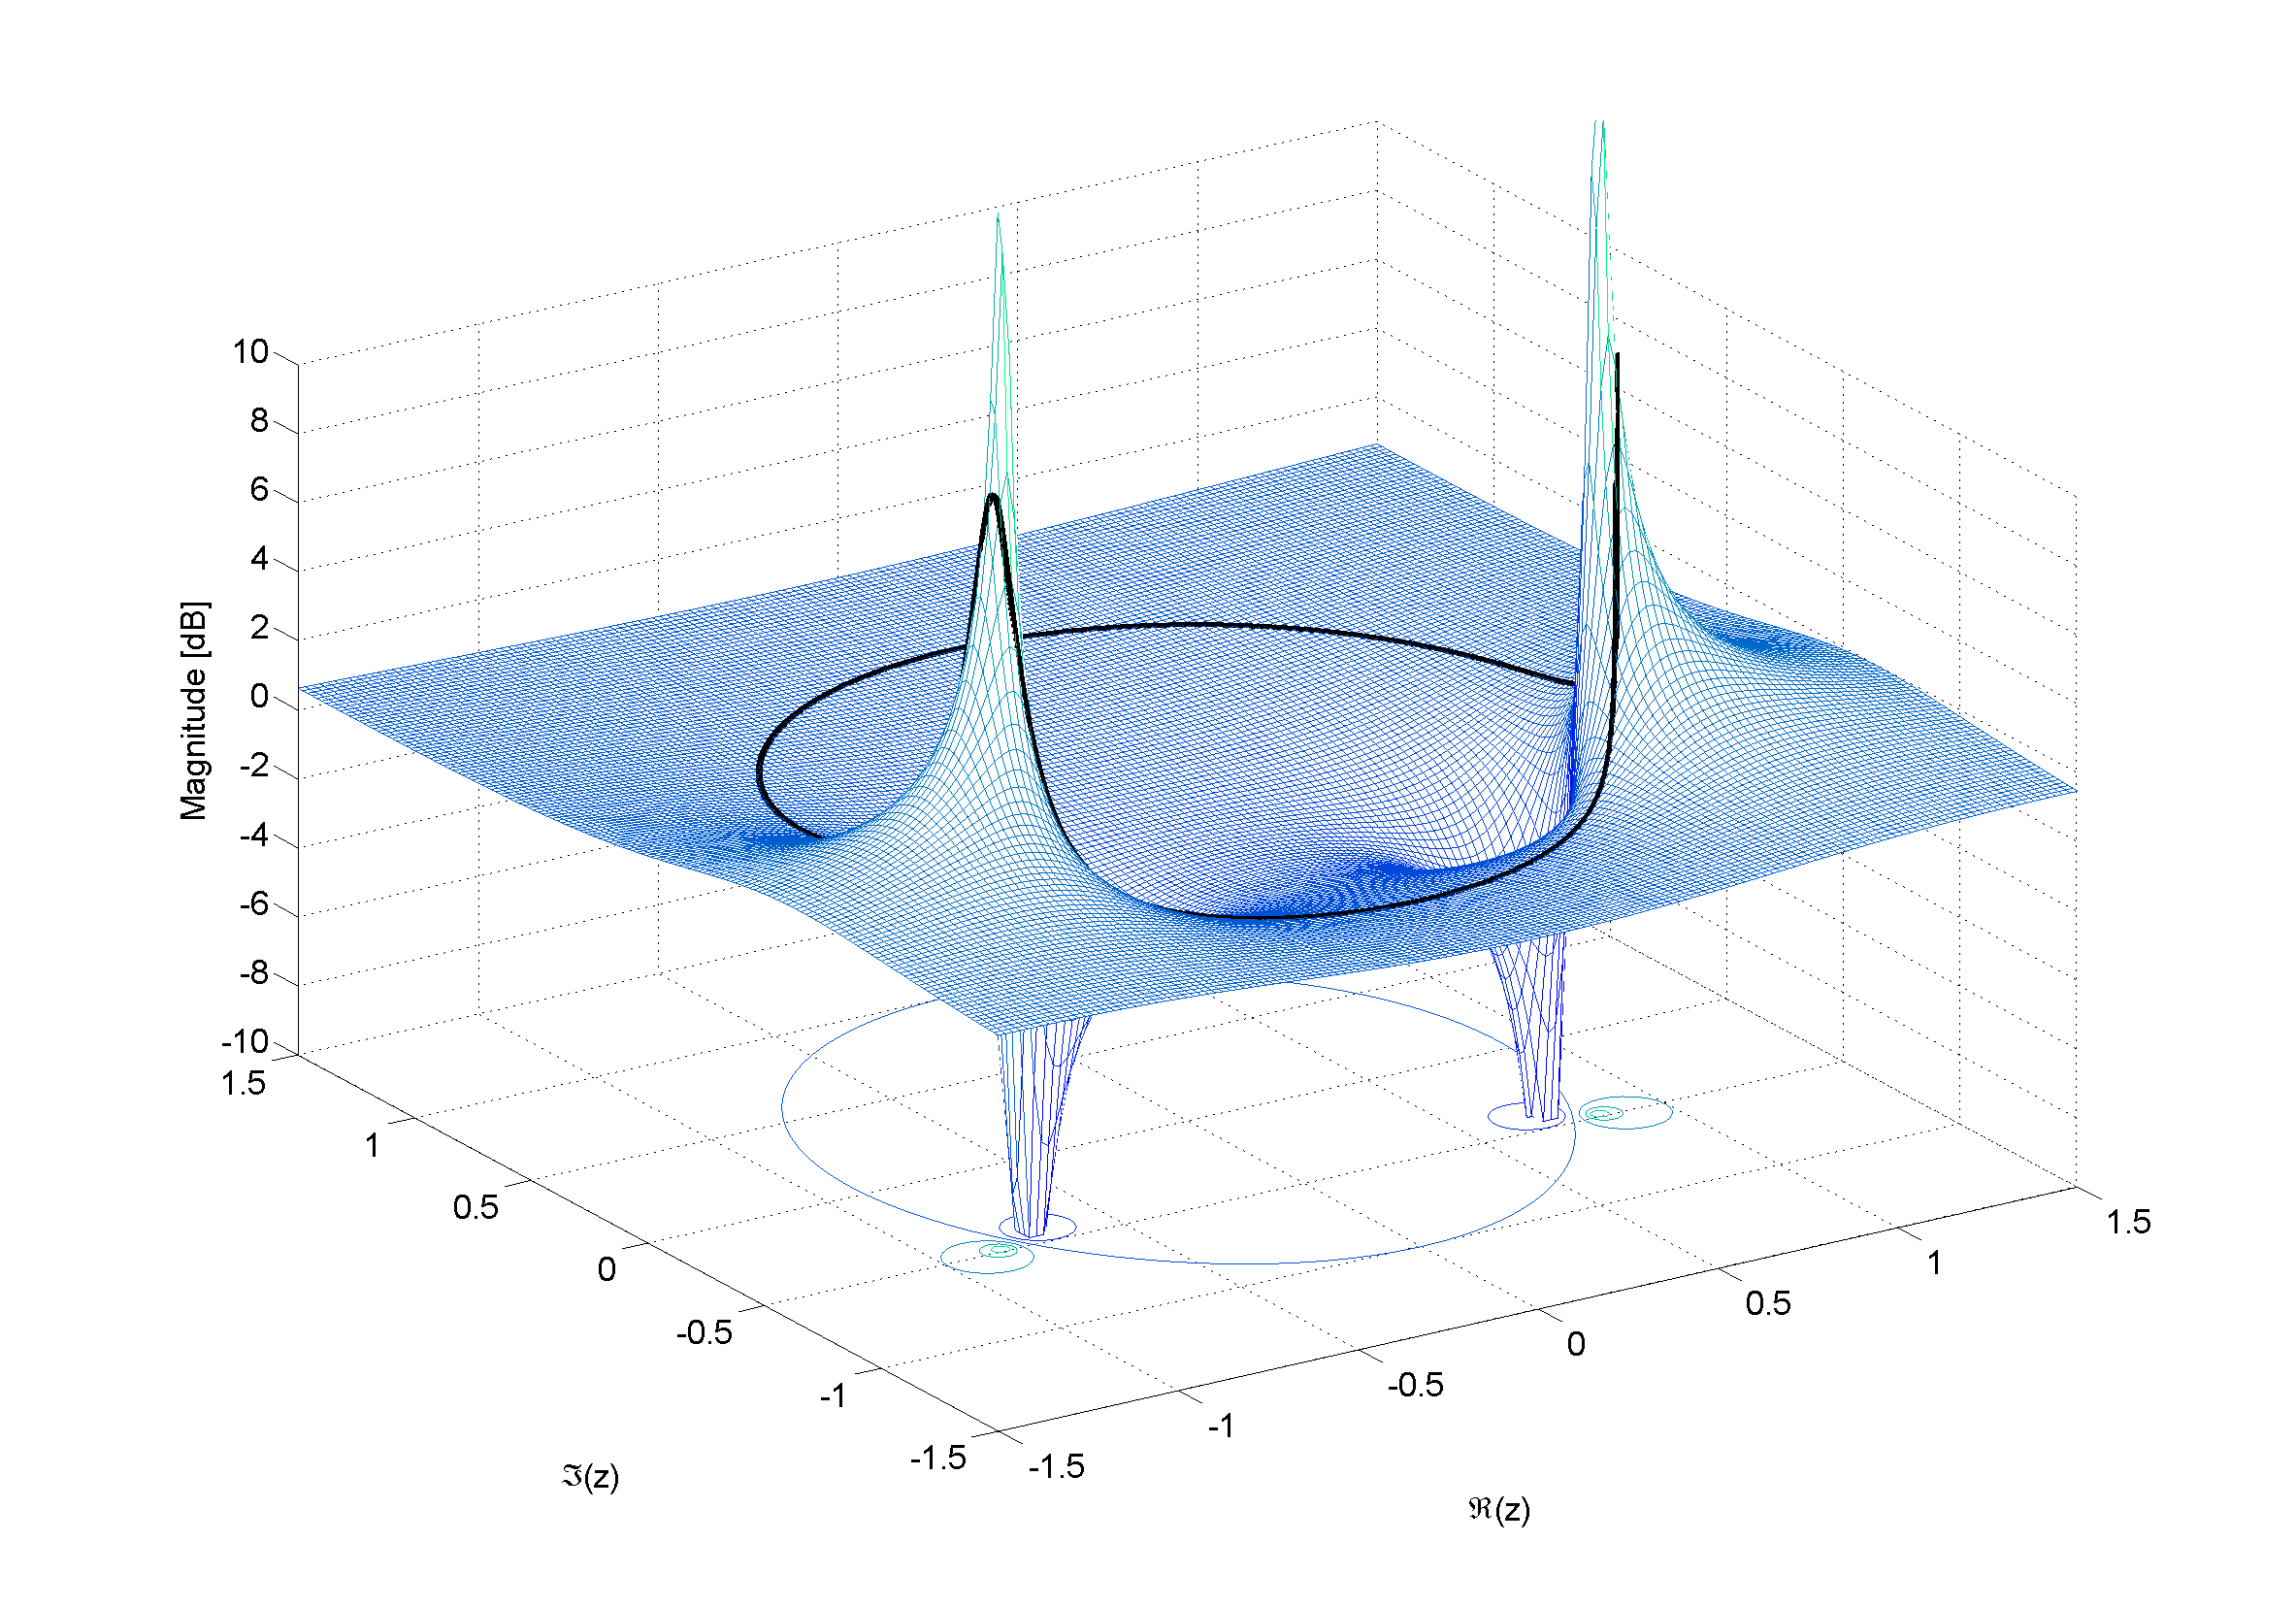
\includegraphics[scale=.26]{graph/PoleZero3d}
					\end{center}
				\end{figure}
 		\end{frame}
		\begin{frame}\frametitle{filters}\framesubtitle{z-transform}
            \begin{equation*}
                X(z) = \sum\limits_{i=-\infty}^\infty x(i)z^{-i}
            \end{equation*}
            \begin{equation*}
                z = \Re\lbrace z \rbrace + \mathrm{j}\Im\lbrace z \rbrace
            \end{equation*}
            \pause
            relation to Fourier transform:
             \begin{equation*}
                X(z)_{|z=e^{\jOm}} = X(\jOm) = \mathfrak{F}\lbrace x(i)\rbrace
            \end{equation*}
 		\end{frame}
		\begin{frame}\frametitle{filters}\framesubtitle{z-plane characteristics}
            \begin{itemize}
                \item   \textbf{stability}:\\ poles within unit circle
                \pause
                \item   \textbf{zero points and poles}\\ are either real or conj. complex
                \pause
                \item   \textbf{minimal phase systems}:\\ no zero points outside of unit circle
                \pause
                \item   \textbf{all pass system}:\\ poles and zeros symmetric wrt unit circle
                \pause
                \item   \textbf{linear phase}:\\ zero points within and outside unit circle symmetric wrt unit circle
            \end{itemize}
 		\end{frame}
\subsection{filter summary}
		\begin{frame}\frametitle{filters}\framesubtitle{FIR \& IIR}
            \begin{table}
                \centering
                    \begin{tabular}{l|cc}
                        & \textbf{FIR} & \textbf{IIR}\\
                        \hline
                        IR length & finite & infinite\\
                        structure & non-recursive & recursive\\
                        phase linearity & possible & impossible\\
                        ratio steepness/workload & low & high\\
                        stability & guaranteed & possibly unstable
                    \end{tabular}
            \end{table}
            \begin{itemize}
                \item   every LTI system is \textbf{completely described} either by
                    \begin{itemize}
                        \item   its complex transfer function,
                        \item   its impulse response, or
                        \item   its pole and zero positions in the z-plane
                    \end{itemize}
            \end{itemize}
 		\end{frame}
		\begin{frame}\frametitle{filters}\framesubtitle{filter design}
            \vspace{-5mm}
            \begin{itemize}
                \item   \textbf{impulse invariance}: sample impulse response
                    \begin{itemize}
                        \item   if continuous system is band-limited, frequency response will be approximately equal (below $\nicefrac{f_\mathrm{S}}{2}$)
                        \item   special case: no filter definition available $\rightarrow$ FIR coefficients 
                    \end{itemize}
                \pause
                \item   \textbf{bi-linear transform}
                    \begin{itemize}
                        \item   map filter from (analogue) Laplace-plane to (digital) z-plane
                        \only<2>{
                            \begin{eqnarray*}
                                s &=& \frac{2}{T}\frac{1-z^{-1}}{1+z^{-1}}\\
                                z &=& \frac{1+s\nicefrac{T_\mathrm{S}}{2}}{1-s\nicefrac{T_\mathrm{S}}{2}}\\
                            \end{eqnarray*}
                        }
                        \item   introduces frequency warping (increasing towards Nyquist frequency)
                    \end{itemize}
                \pause
                \item   \textbf{frequency transformation}
                    \begin{itemize}
                        \item   transform a (low-pass) prototype filter
                        \item   usually via all-pass mapping filter
                    \end{itemize}
                \pause
                \item   \textbf{iterative approximation} of the magnitude response
                \pause
                \item   \textbf{intuitive methods}
                    \begin{itemize}
                        \item   manually move zeros and poles in z-plane
                        \item   draw magnitude response in frequency domain
                    \end{itemize}
            \end{itemize}
 		\end{frame}
		\begin{frame}\frametitle{filters}\framesubtitle{effects of word length}
            \vspace{-5mm}
            \begin{itemize}
                \item   quantization of filter coefficients can lead to problems
                \item   effects depend on filter type and structure:
                    \begin{itemize}
                        \item   changes of transfer function
                        \item   instability
                        \item   quantization noise $\rightarrow$ SNR
                    \end{itemize}
            \end{itemize}
			\vspace{-3mm}
            \only<2>{
				\begin{figure}[!hbt]
					\begin{center}
						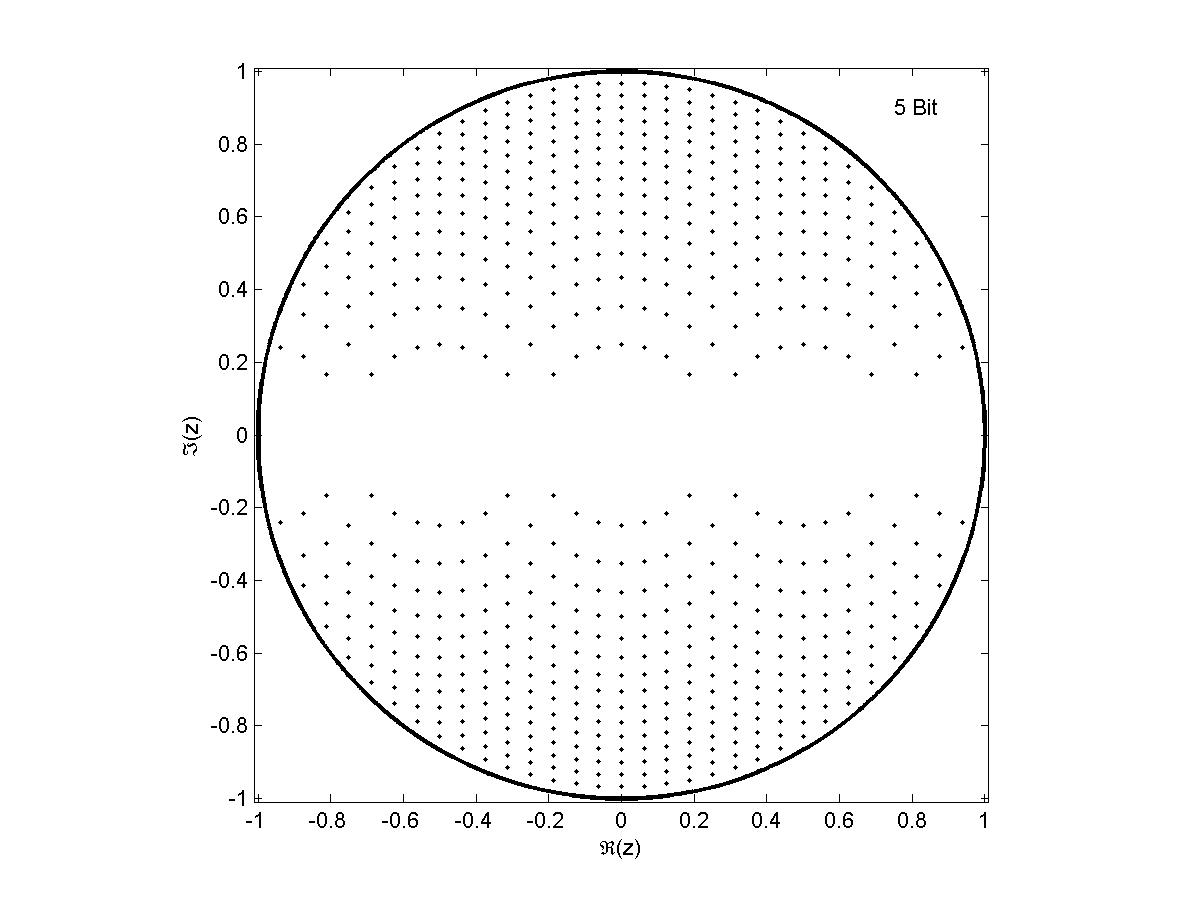
\includegraphics[scale=.35]{graph/QuantPolePlotDirect_1}
					\end{center}
				\end{figure}
			}
			\only<3>{
				\begin{figure}[!hbt]
					\begin{center}
						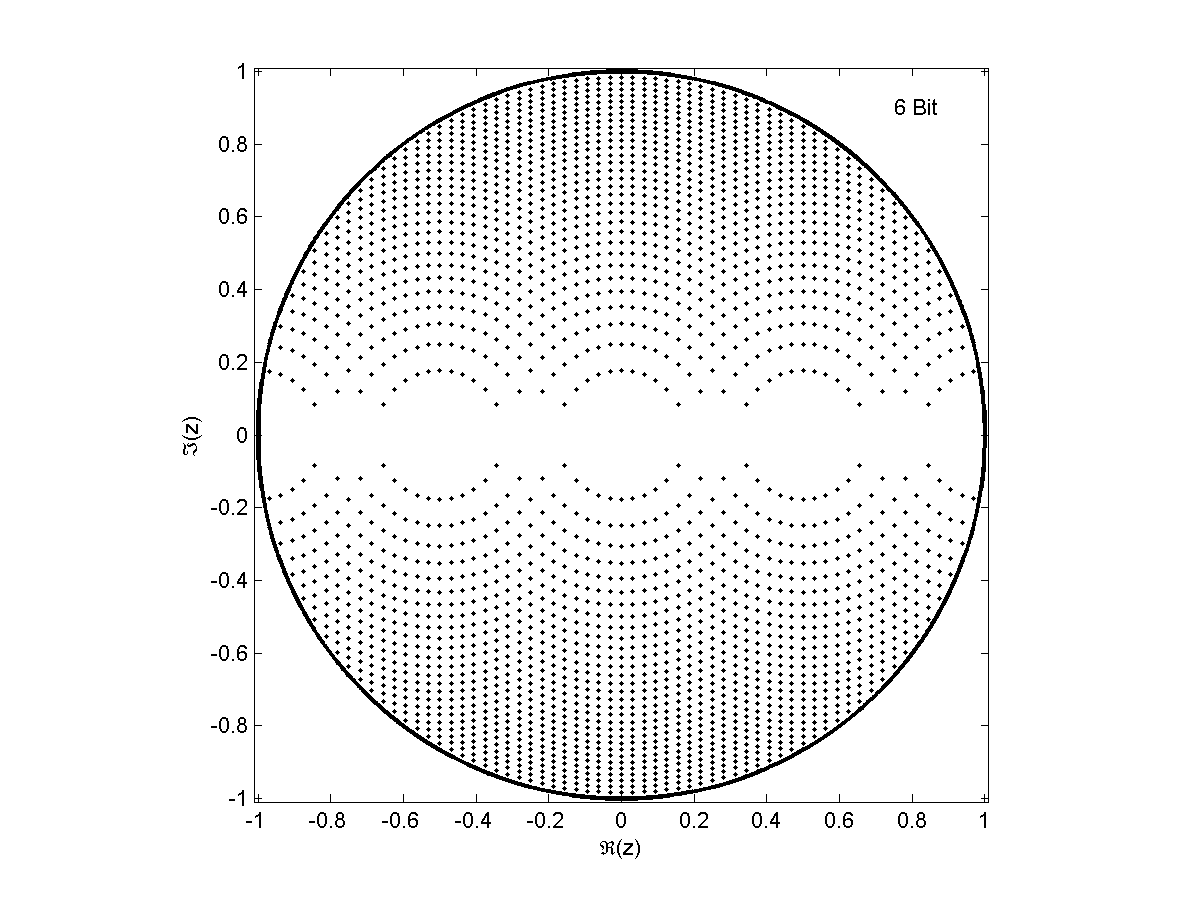
\includegraphics[scale=.35]{graph/QuantPolePlotDirect_2}
					\end{center}
				\end{figure}
			}
			\only<4>{
				\begin{figure}[!hbt]
					\begin{center}
						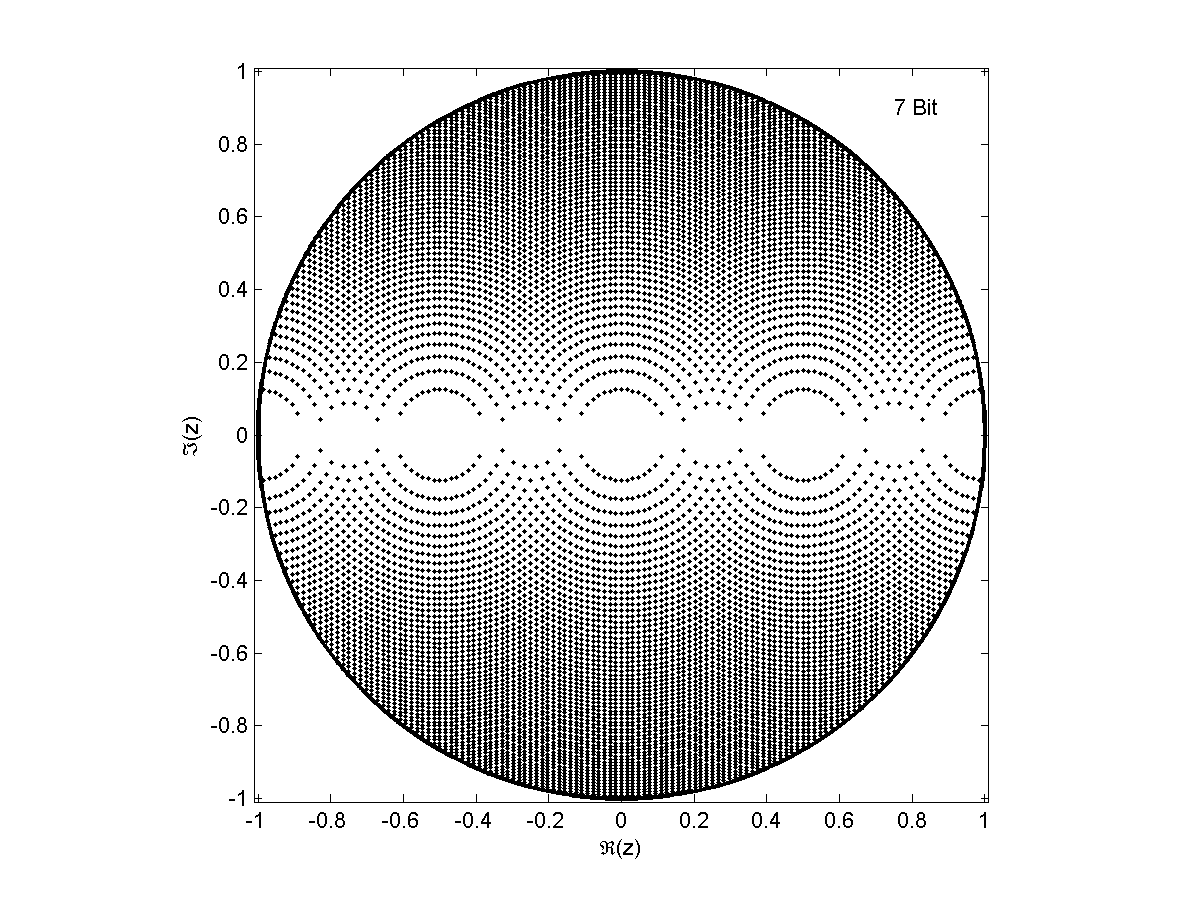
\includegraphics[scale=.35]{graph/QuantPolePlotDirect_3}
					\end{center}
				\end{figure}
			}
			\only<5>{
				\begin{figure}[!hbt]
					\begin{center}
						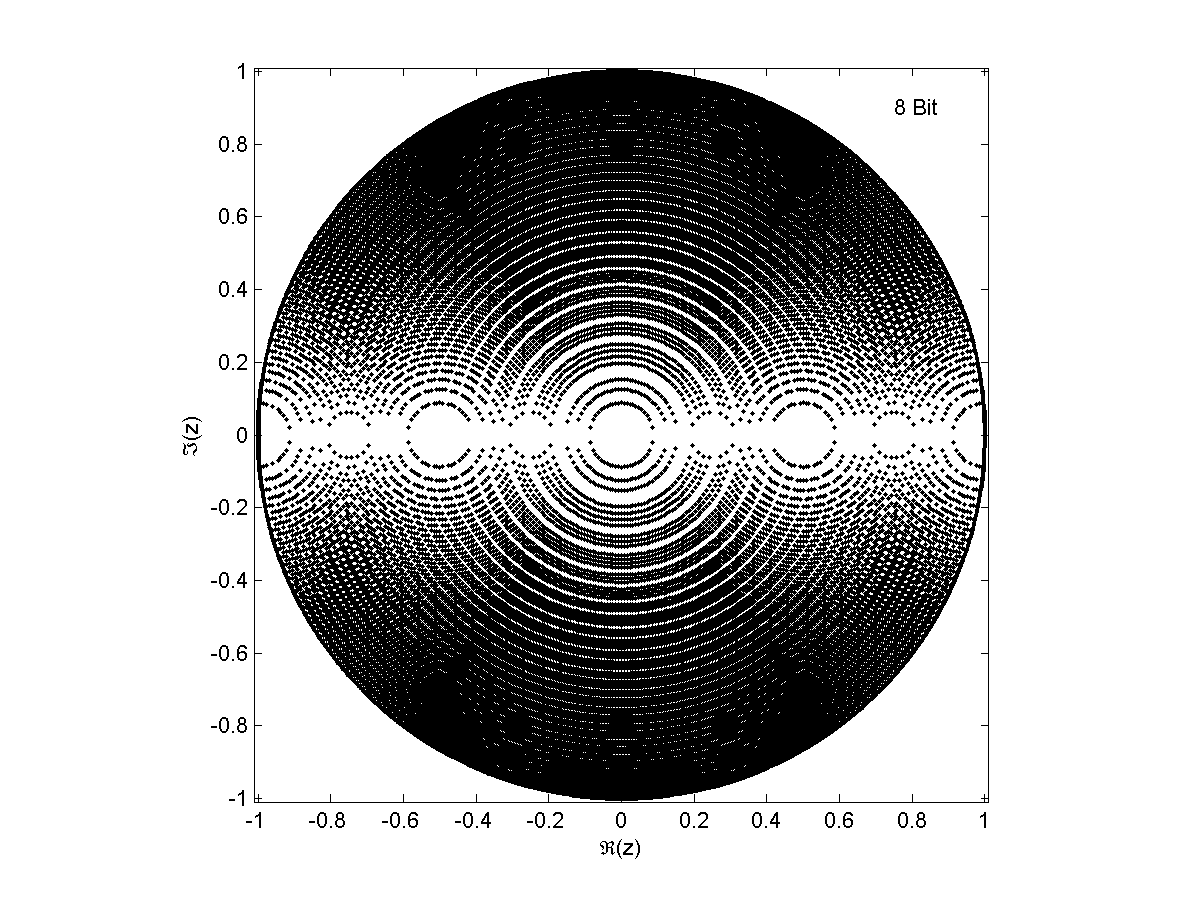
\includegraphics[scale=.35]{graph/QuantPolePlotDirect_4}
					\end{center}
				\end{figure}
			}
            \vspace{50mm}
 		\end{frame}
		\begin{frame}\frametitle{filters}\framesubtitle{convergence of the z-transform 1/3}
            \begin{itemize}
                \item definition
                \begin{footnotesize}
                \begin{equation*}
                    X(z) = \sum\limits_{i=-\infty}^\infty x(i)z^{-i}
                \end{equation*}
                \end{footnotesize}
                \pause
                \item   stability
                \begin{footnotesize}
                 \begin{equation*}
                    |X(z)| = \left|\sum\limits_{i=-\infty}^\infty x(i)z^{-i}\right| \leq \sum\limits_{i=-\infty}^\infty |x(i)||z|^{-i} \leq \infty
                \end{equation*}
                 \end{footnotesize}
                   \begin{enumerate}
                        \item   right side: $\lim\limits_{N\rightarrow\infty}\sum\limits_{i=0}^N x(i)z^{-i}$ converges for $|z| > R_1$
                        \pause
                        \item   left side: $\lim\limits_{N\rightarrow\infty}\sum\limits_{i=-\infty}^{-1} x(i)z^{-i}=\lim\limits_{N\rightarrow\infty}\sum\limits_{n=1}^{N} x(-n)z^{n}$ converges for $|z| < R_2$
                    \end{enumerate}
           \end{itemize}
 		\end{frame}
		\begin{frame}\frametitle{filters}\framesubtitle{convergence of the z-transform 2/3}
            \begin{equation*}
                \text{Region of Convergence (ROC): } R_1\leq |z| \leq R_2
            \end{equation*}
            \pause
            
            \begin{itemize}
                \item                 \textbf{observations}
                \begin{itemize}
                    \item   $R_1,R_2$ define circles
                    \item   $R_1 > R_2$: z-transform does not exist
                    \item   causality: $R_2 \rightarrow \infty$
                \end{itemize}
                \item   \textbf{properties}
                    \begin{itemize}
                        \item   ROC cannot contain poles, boundaries include poles (or are at $0, \infty$)
                        \item   since we need $|H(\jOm)|$ to exist, $R_1 \leq 1$!
                    \end{itemize}
            \end{itemize}
 		\end{frame}
		\begin{frame}\frametitle{filters}\framesubtitle{convergence of the z-transform 3/3}
            \begin{figure}
                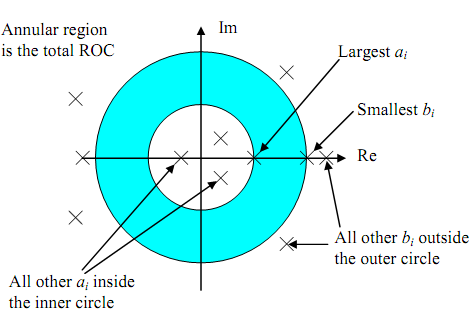
\includegraphics[scale=.8]{graph/ROC}
            \end{figure}
 		\end{frame}
		\begin{frame}\frametitle{filters}\framesubtitle{convergence example}
            example: damped sinusoidal $ h(i) = R^i e^{\jom iT}$
            \begin{eqnarray*}
                H(z) &=& \sum\limits_{n=0}^\infty  R^n e^{\jom nT}z^{-n}\\
                &=& \sum\limits_{n=0}^\infty  \left(R e^{\jom nT}z^{-1}\right)^n\\
                \pause
                &=& \frac{1}{1-R e^{\jom nT}z^{-1}}
            \end{eqnarray*}
            
            \begin{itemize}
                \item   single pole at $z=Re^{\jom T}$
                \item   exists for $|z| > R$ \pause $\Rightarrow$ since it has to exist on the unit circle, $|z| < 1$
            \end{itemize}
        \end{frame}
       
